\documentclass[conference]{IEEEtran}
\IEEEoverridecommandlockouts
% The preceding line is only needed to identify funding in the first footnote. If that is unneeded, please comment it out.
\usepackage{cite}
\usepackage{amsmath,amssymb,amsfonts}
\usepackage{algorithmic}
\usepackage{graphicx}
\usepackage{textcomp}
\usepackage{xcolor}
\def\BibTeX{{\rm B\kern-.05em{\sc i\kern-.025em b}\kern-.08em
    T\kern-.1667em\lower.7ex\hbox{E}\kern-.125emX}}
\begin{document}

\title{Data Structures*\\
%{\footnotesize \textsuperscript{*}Note: Sub-titles are not captured in Xplore and
%should not be used}
%\thanks{Identify applicable funding agency here. If none, delete this.}
}

\author
{\IEEEauthorblockN{1\textsuperscript{st} Sarvesh Anant Kulkarni}
\IEEEauthorblockA{\textit{Computer Engineering} \\
\textit{COEP Technological University}\\
Pune India \\
email : kulkarnisa22.comp@coep.ac.in}


}

\maketitle

\begin{abstract}
This document is a model and instructions for \LaTeX.
This and the IEEEtran.cls file define the components of your paper [title, text, heads, etc.]. *CRITICAL: Do Not Use Symbols, Special Characters, Footnotes, 
or Math in Paper Title or Abstract.
\end{abstract}

\begin{IEEEkeywords}
component, formatting, style, styling, insert
\end{IEEEkeywords}

\section{Introduction}
This report is for those enthusiastics who are eager to explore data structures.

\section{Choosing a Data Structure/Algorithm
	}

\subsection{Maintaining the Integrity of the Specifications}
\paragraph{
The choice of data structure or algorithm to cover is largely open ended. But you must send a short paragraph explaining your plan before Thanksgiving break. This should include the topic you plan to cover and what you aim to discuss in your paper. }
\paragraph{
You can use the book to find example data structures that we did not cover, or explore resources online. While Wikipedia is not a primary source, it is a reliable repository of data structures that can be easily explored and there are usually good examples.}




\section{Writeup Requirements}
Your writeup should be well-structured and follow scientific writing principles. You can structure as you see fit, but at a minimum, your paper should include:

\begin{enumerate}

  \item An introduction - this can include a history and a preview of the central features of the data structure/algorithm
  \item Motivation - what is the problem that needs to be solved? It is recommended that you come up with real-world application and describe it here.
  \item Background/related work - what does this relate to from class? What are the conceptual differences? Are there other algorithms/data structures that generally compete with your choice?	
  \item Interface - what are the major operations of the data structure? This may not apply for an algorithm, but you discuss assumptions for the structure of the data.
  \item Illustration - walk through an example (e.g., for BFS, going from Parrish to the Ville). You should have some sort of diagram that illustrates how the data structure/algorithm works.
  ~\cite{da} 
  \item Analysis - provide pseudocode for a few key operations and analyze their run time. This does not need to be exhaustive, and how many operations you cover depends on the complexity of the problem. For example, inserting/removing from linked lists was fairly simple so it would be good to cover most of the methods. Removing/inserting into an AVL tree is quite complex, so be sure to limit your discussion to one or two key operations. You should then summarize the other operations.
~\cite{ds} 

\end{enumerate}


\subsection{Presentation}\label{AA}
You will present your findings in a short presentation (maximum 12 minutes) during lecture on Tuesday, December 10. You will be divided into groups of 10 students with one discussion leader (Prof. Soni, Prof. Brody, a ninja, or Frances). Each student in your group as well as the discussion leader will evaluate your presentation on the criteria defined.

\subsection{Logistics and Tips}
\begin{itemize}
\item You are permitted to use powerpoint/slides if you like. This has been rare in the past as making slides is time consuming. But if you choose to use any visualization requiring a projector, you must let me know ASAP. Also, you should show up a few minutes early to set up your laptop.
\item Some students in the past have provided a worksheet to help in their presentation, or to supplement their presentation with more details that had tobe omitted due to time.
\item Be sure to practice! 12 minutes goes by much faster than you'll expect
\item Do not try to cover every aspect of your topic. Specifically, the presentation does not need to cover all the aspects of your paper.
\item Moreover, a good strategy is to concentrate on one sub-problem and give a high-level intuition of other topics.
\end{itemize}

\subsection{Basics of Data strucutre}
A data structure is a storage that is used to store and organize data. It is a way of arranging data on a computer so that it can be accessed and updated efficiently.

\begin{itemize}
\item Linear data structure: Data structure in which data elements are arranged sequentially or linearly, where each element is attached to its previous and next adjacent elements, is called a linear data structure. 
  
\begin{itemize}
\item Static data structure: Static data structure has a fixed memory size. It is easier to access the elements in a static data structure. 
An example of this data structure is an array.
\item Dynamic data structure: In dynamic data structure, the size is not fixed. It can be randomly updated during the runtime which may be considered efficient concerning the memory (space) complexity of the code. 
Examples of this data structure are queue, stack, etc.
\end{itemize}
Non-linear data structure: Data structures where data elements are not placed sequentially or linearly are called non-linear data structures. In a non-linear data structure, we can’t traverse all the elements in a single run only. 
Examples of non-linear data structures are trees and graphs.
\end{itemize}


\subsection{Why Learn Data Structures and Algorithms?}

This article is for those who have just started learning algorithms and wondered how impactful it will be to boost their career/programming skills. It is also for those who wonder why big companies like Google, Facebook, and Amazon hire programmers who are exceptionally good at optimizing Algorithms.


\subsection{Asymptotic Analysis: Big-O Notation and More}\label{SCM}
In this tutorial, you will learn what asymptotic notations are. Also, you will learn about Big-O notation, Theta notation and Omega notation.

The efficiency of an algorithm depends on the amount of time, storage and other resources required to execute the algorithm. The efficiency is measured with the help of asymptotic notations.

An algorithm may not have the same performance for different types of inputs. With the increase in the input size, the performance will change.

The study of change in performance of the algorithm with the change in the order of the input size is defined as asymptotic analysis.

\subsection{Authors and Affiliations}
\textbf{The class file is designed for, but not limited to, six authors.} A 
minimum of one author is required for all conference articles. Author names 
should be listed starting from left to right and then moving down to the 
next line. This is the author sequence that will be used in future citations 
and by indexing services. Names should not be listed in columns nor group by 
affiliation. Please keep your affiliations as succinct as possible (for 
example, do not differentiate among departments of the same organization).

\subsection{Asymptotic Notations}
symptotic notations are the mathematical notations used to describe the running time of an algorithm when the input tends towards a particular value or a limiting value.

For example: In bubble sort, when the input array is already sorted, the time taken by the algorithm is linear i.e. the best case.

But, when the input array is in reverse condition, the algorithm takes the maximum time (quadratic) to sort the elements i.e. the worst case.

When the input array is neither sorted nor in reverse order, then it takes average time. These durations are denoted using asymptotic notations.

There are mainly three asymptotic notations:


\begin{itemize}
\item Big-O notation
\item Omega notation
\item Theta notation
\end{itemize}
 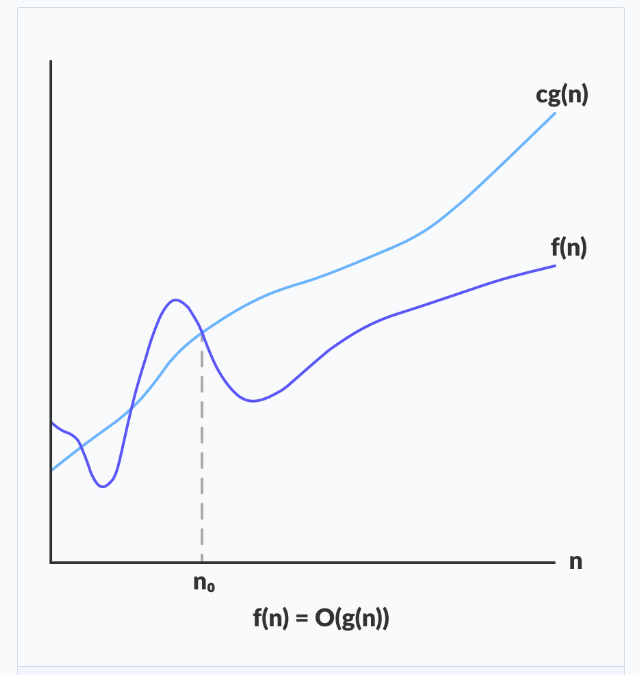
\includegraphics[width=\linewidth]{1.png}
 
  \label{fig:DSA Complexity}
The above expression can be described as a function f(n) belongs to the set O(g(n)) if there exists a positive constant c such that it lies between 0 and cg(n), for sufficiently large n.

For any value of n, the running time of an algorithm does not cross the time provided by O(g(n)).


\section*{}


\begin{thebibliography} {}

\bibitem{da} “C++: The Complete Reference”, Herbert Schildt, Fourth Edition, 2002, The McGrawHill company, ISBN 0-07-222680-3
\item “Fundamentals of Data Structures in C++”, Ellis Horowitz, S. Sahni, D. Mehta, 2nd
Edition, 2008, University Press, ISBN-10: 8173716064
\bibitem{ds}“An introduction to data structures with Applications”, Jean-Paul Tremblay, Paul. G.
Soresan, 2nd Edition, 1984, Tata Mc-Graw Hill International Editions, ISBN-0-07-
462471-7


\end{thebibliography} 




\end{document}
